\chapter{Existing Approaches in Behavior Analysis and Detection of Customer Satisfaction}
\label{ch:backgroundResearch}

\section{Interpretation of Customer satisfaction}
The beginning of research work in terms of measuring and analyzing how satisfied users are with a computer system already dates back to the beginning of the 80s. At these times first researchers supposed that there is a relationship between user satisfaction and the success of a computer system. From this point on, a series of researches investigated which factors could influence user satisfaction and how to ask users to get a representative opinion \cite{roy1998developing}. Bailey \& Pearson were first to propose a questionnaire consisting of 39 satisfaction dimensions which should help information system providers to evaluate whether a user is satisfied with the system or not. Ives, Olsen \& Baroudi did some further research based on the existing work from Bailey \& Pearson to reduce the effort for users to answer 39 dimensions. However technology changed dramatically as the shift towards the use of personal computers started a few years later and therefore new approaches were needed. According to Doll and Torkzadeh the previous developed methods did not focus on the satisfaction with a specific end-user application since they do not cover the human-machine interaction \cite{roy1998developing}. Thus, they developed a model specifying the end-user satisfaction as a second factor driven by five first-order factors namely content, format, accuracy, timeliness and ease of use. After testing four different models regarding validity and reliability using a confirmatory factor analysis approach against some sample data, they came up with the following model visualized in figure ~\ref{fig:relatedDoll}. 

\begin{figure}
	\centering
	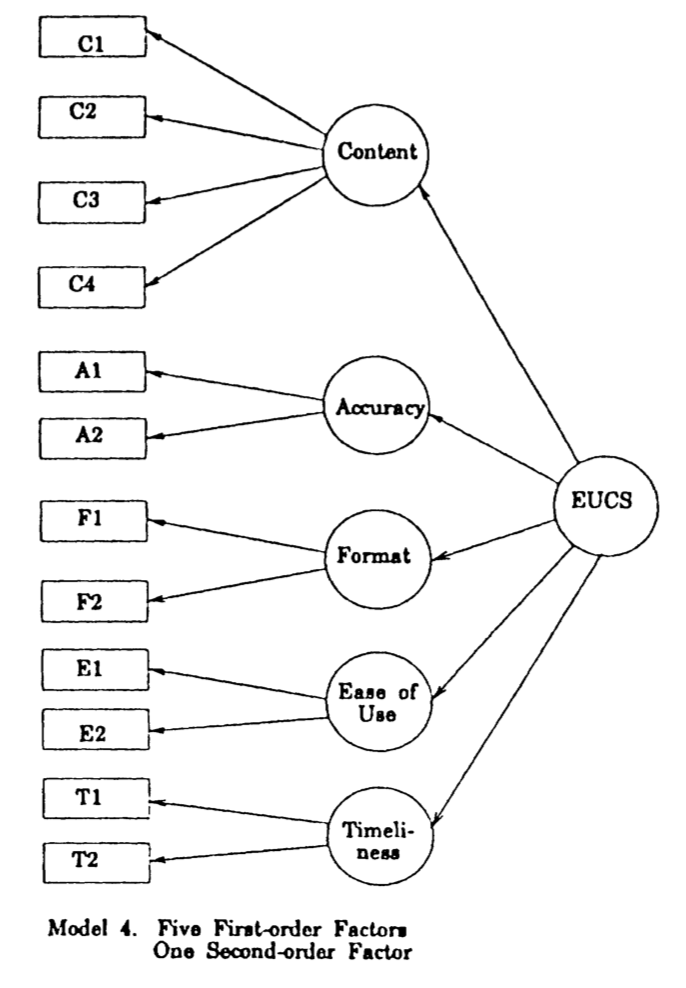
\includegraphics[width=1.0\textwidth]{img/dollSecondFactor.png}
	\caption{Customer Satisfaction - Five first-order factors \cite{doll1994confirmatory}}
	\label{fig:relatedDoll}
\end{figure} 

In the results for this model they claim that 74\% of the variation in the five first-order factors is explained by the end-user satisfaction. \cite{doll1994confirmatory}. This second-factor approach turned out to be quite successful over the following years and has been widely used to reason about user satisfaction for specific applications. The web has been evolving rapidly and due to this reason \cite{xiao2002measurement} analyzed in their research in 2002 whether the existing method of Doll and Torkzadeh is still appropriate and applicable to web-based information systems. They recognized that some of the previously identified factors may not be relevant anymore for web-based information systems. Based on the work of Doll and Torkzadeh, a questionnaire was created to ask people how satisfied they are with a web based information system whereby they decided to choose Internet Portals as representative example. The results of this research showed that the existing five factors are still valid under these new circumstances. However, the research clearly has some limitations as it only considered Internet Portals and did not look on additional factors like privacy or security \cite{xiao2002measurement}. In 1999 \cite{roy1998developing} took a closer look on several existing measurement approaches and discussed their limitations in practice. In contrast to \cite{xiao2002measurement} the results of this research tend to be more critical regarding practical usefulness of approaches like the one from Doll and Torkzadeh. They criticize that surveyed users are considered with equal personality and behavior whereas in practice each individual user is different and this would therefore require an independent consideration in a survey. Furthermore the research claims that existing survey approaches are often too inflexible since a service provider has specific objectives and the survey has to put more focus on certain aspects than others which cannot be achieved without modifications. Meanwhile researchers recognized that besides extracting knowledge about customer satisfaction explicitly, there is another promising opportunity to implicitly understand behavior of customers based on how they present themselves, act and behave. Supported by the rapid growth of software technology and tools the era of statistical analysis and data mining in CRM started up in the beginning of the 21st century \cite{Ngai2009} \cite{neckel2015}. The research paper of \cite{Ngai2009} wrapped up CRM quite comprehensively by taking a closer look onto 87 selected published journals dealing with CRM and Data Mining techniques. They tried to find out how the distribution of publications among the different areas of CRM looks like and as a result came to the conclusion that statistical and data mining techniques are especially in customer retention of great interest. A promising approach reasoning about dissatisfaction of customers and its connection to churn was proposed by \cite{mozer2000predicting}. This research project first of all analyzed influencing factors driving customers in the wireless telecommunications industry to stay or leave the service. After identifying major factors differentiating between satisfied and dissatisfied customers, statistical machine learning techniques as logistic regression, decision trees and neural networks were employed to predict churn rate for a selected time period. Later on \cite{mozer2000predicting} outlines a calculation model to determine under which circumstances it makes sense to offer an incentive to a potential churner and take the opportunity to pursue him/her to stay. Based on the variables of lost revenue due to a churner, acquisition costs of a new customer, the probability of staying after offered an incentive and the cost of offering an incentive to a customer, an cost saving per customer could be calculated. The results clearly showed that in most cases taking the effort of offering incentives and thus preventing churn results in higher profitability. Due to the similarity, considering the recurring payment service type as well as properties and nature of competition on the market, with the illustration example outlined in~\ref{sec:illustrationExample}, the research of \cite{mozer2000predicting} supports the practical work conveyed by this thesis. Another related research work published by \cite{lariviere2005predicting} dealt with analysis of customer behavior and its impact on retention and profitability for a European Financial Institute. Using a data set of about 100k customers and advanced decision tree algorithm, namely Random Forest, was employed to perform a binary classification based on the properties of whether a customer
\begin{itemize}
	\item buys a further banking product in the future,
	\item cancels a non-ending relationship with a purchased product,
	\item or causes a profit drop within a considered time period.
\end{itemize}
In a further stage the Random Forest algorithm was also used to analyze which of the identified independent variables affect the outcome factors related to customer retention remarkably. As surprising side effect it was found out that some of the variables show an influencing effect in all three binary classifiers although they seem quite contrary as the new-buy and cancellation of a product for instance. 

The previous work from \cite{mozer2000predicting} and \cite{lariviere2005predicting} already shows the power of statistical and machine learning techniques to predict future customer behavior and its effect on retention and profitability. It was clearly indicated that past customer behavior data turns out to be worthy in recognizing patterns, relationships and predicting the future. Since customer satisfaction is usually a rather complex construct consisting of several dimensions besides purchase, cancellation and profit evolution of a product, there is enough potential to reveal hidden patterns and answer business critical questions regarding customers behavior. Moreover statistical tools and data mining techniques have evolved further and demand for a reappraisal. According to \cite{gantz2012digital} only half a percent of the data available in the digital universe is analyzed but in 2020 about 33\% of all data may be valuable which supports the assumption that there is still a lot of work ahead. 

\section{Concepts}
Analyzing a customer's attitude towards a product, recognizing whether his/her expectations are met and providing the desired value at the needed time, is usually a difficult challenge and requires a company to setup a well coordinated working process. \cite{Ngai2009} illustrated CRM as a framework comprising four core dimensions whereby on each of them, integration of knowledge about customers can be used to increase company profitability \cite{neckel2015}. Before looking in greater detail on the technical concepts of how to organize collected data about customers and finding useful information hidden in those large datasets, the thesis will take a look on the CRM dimensions proposed by \cite{swift2001accelerating}. The aim is to outline the various tasks of CRM but also clearly mark out at which particular dimension(s) the focus of this thesis lies. 

\subsection{Customer Identification}
No successful company launched their first product and immediately interested customers recognized the potential of the product and bought it. In contrast potential customers first of all have to be found by a careful segmentation following by an analysis of these identified segments which should lead to concrete customer segments one wants to target \cite{swift2001accelerating} \cite{Ngai2009}. 

\subsection{Customer Attraction}
The concept of attracting customers as a major prerequisite to develop trust and commitment between a seller and a buyer has already been outlined by \cite{dwyer1987developing} in 1987. The goal of this part in the CRM Framework is to raise attention by potential customers and present outstanding features and differentiators of the product which lead to fulfilling needs of the customer \cite{ellegaard2006customer}. 


